% In your report, answer the following questions.

% A. Discuss the advantage/problem/limitation of RANSAC for estimating the fundamental matrix.

% B. Analyze the difference in results as each RANSAC parameter changes.
% (Inlier distance, number of iteration etc..)

% C. [BONUS] Analyze the difference in results as each method changes.
% (Feature extraction methods, feature matching methods, RANSAC variants, distance measures
% etc..)

\section{Suitability of RANSAC for fundamental matrix estimation}

As always, RANSAC's number 1 problem is it's random, iterative nature; It can't
guarantee a good fit, although it usually finds one, especially in better
implementations of the algorithm. In mine, however, I find the results to vary
too much. Sometimes a run produces unusable results, other times they're
near-perfect. RANSAC parameters might also need tweaking depending on the image
properties, for example the ratio of inliers to outliers.

However, there are advantages to using RANSAC for the fundamental matrix
estimation. One is that we only use 7 point correspondences, and thus there's
no need to force the matrix into a rank 2 form, unlike in the linear
algorithms. Another advantage is that RANSAC is a widely used, simple, and well
understood algorithm, which simplifies application.

\subsection{Effect of RANSAC parameters}

The iteration count didn't seem to have too big of an effect on results.
Usually after 500 iterations all the inliers were found, often even after 200.

The distance threshold had a big effect on the results. However, for some
reason I got very large Sampson errors, I had to use a threshold of up to 500.
Which seems strange, because I thought the distance threshold should be
somewhere between 1 and 10, or below 100 at least. Probably there's some errors
in my error calculations.

\section{Results}

I have to admit that none of my results were too good. I couldn't quite seem to
make the algorithm work as I expected it to. I don't know if the problem was
with the detected features, my Sampson error calculation, the calculation of
the fundamental matrix, a random bug or something else. Still, here are some of
my results.

\begin{figure}[h]
  \centering
  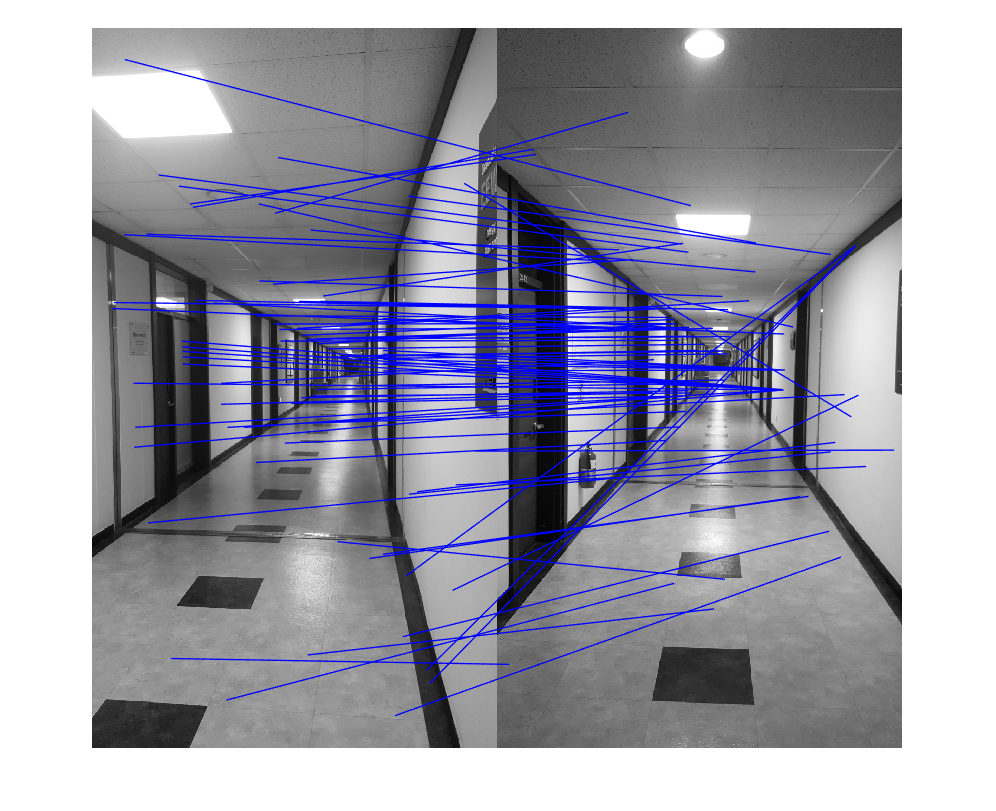
\includegraphics[width=0.8\linewidth]{inlier_matches}
  \caption{RANSAC inlier matches. Clear mismatches visible.}\label{fig:}
\end{figure}

\begin{figure}[h]
  \centering
  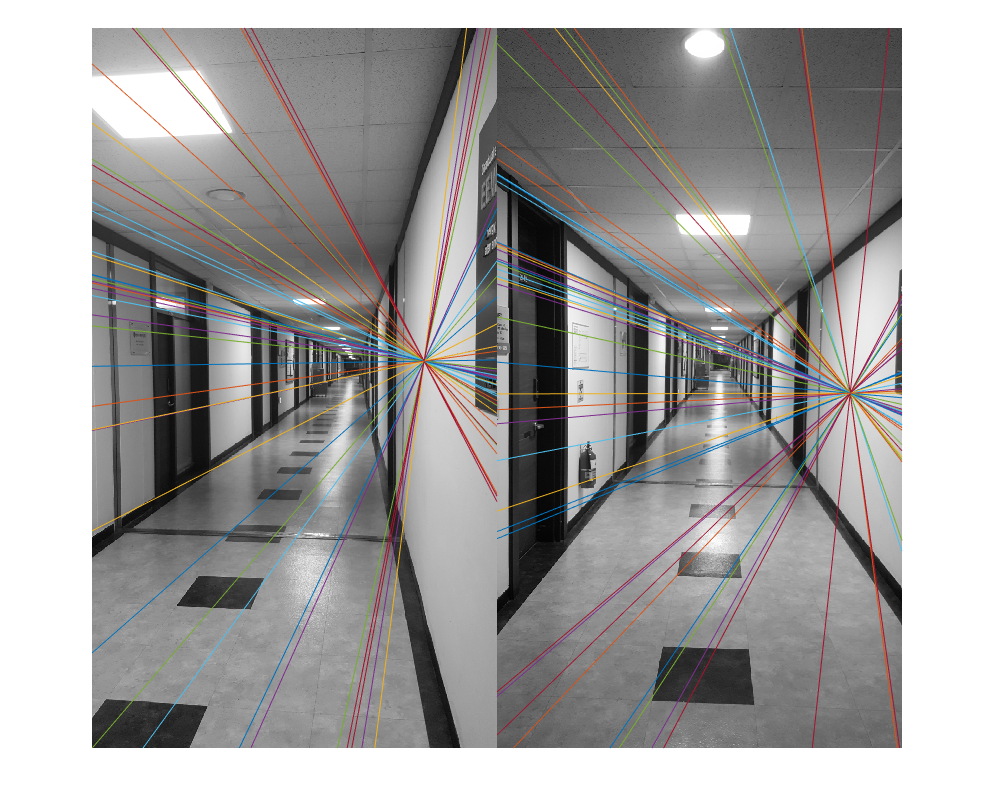
\includegraphics[width=0.8\linewidth]{lm_epipoles}
  \caption{Epipolar lines calculated from the Levenberg-Marquadt optimized
  fundamental matrix.}\label{fig:}
\end{figure}

\begin{figure}[h]
  \centering
  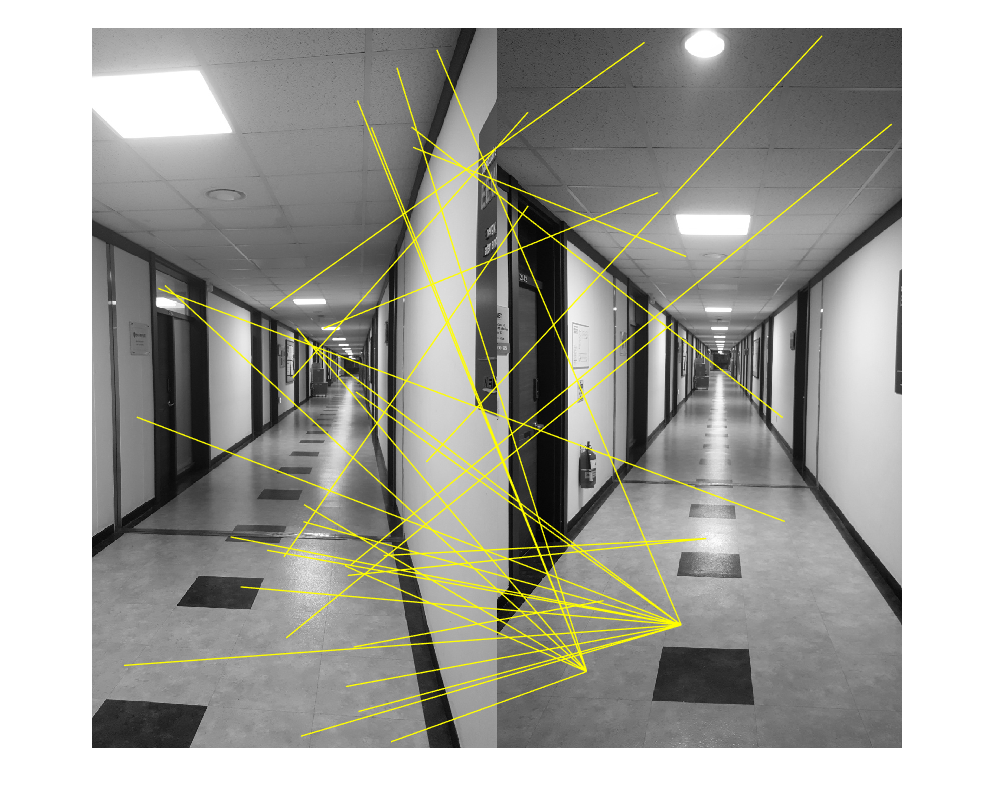
\includegraphics[width=0.8\linewidth]{guided_matches}
  \caption{Guided matches using the epilines. Unfortunately they're quite bad.}\label{fig:}
\end{figure}
